\documentclass[10pt]{article}
\usepackage{amsmath}
\usepackage{graphicx}

\setlength{\textheight}{8.5in}
\setlength{\topmargin}{0in}
\setlength{\textwidth}{6.25in}
\setlength{\oddsidemargin}{0.125in}
\setlength{\evensidemargin}{0.125in}

\begin{document}

\centerline{\sc \large Modeling visual numerosity with deep learning } %Title
\vspace{.5pc}
%\centerline{\sc Rotation project with Professor Jay McClelland} %author/subtitle
\centerline{\sc}
\vspace{3pc}
\setlength\parindent{0in}
\section{Introduction}
We investigate the illustration of `visual number sense' in deep hierarchical models, by Zorzi et. al.. By building a multi-layer Deep Belief Network, the authors show that it is possible to extract features with a sense of basic numerosity in the range of integers 1 to 32. More specifically, using features in deeper network layers, it is possible to linearly classify integers below or above 8 (or 16) with fair accuracy. This indicates that the population of neurons in the deep layer produce numerosity features. Further, the weber ratio calculated from representative numerosity neurons were estimated (w=0.15) to be similar to that of human adults. This results correlates well with cognitive studies of animals and humans \cite{Piazza04}, which indicate that numerical sense and competency do not emerge with linguistic or symbolic understanding, but rather, can be understood as a built-in biological function\cite{Nieder05}. 

This short document attempts to reproduce results of Zorzi et. al. with hierarchical neural networks. We systematically record and analyze their results, and provide reference for on-going projects on cognitive number sense. 

\section{Training data}
The data in Zorzi et. al. contains binary visual data containing squares of different areas, randomly positioned in the visual field. According to details in their supplementary materials, the data generation process was exactly reproduced. An example is shown in Figure~\ref{fig:train_data}.

\begin{figure}[tbh]
\centering
\includegraphics[width=0.4\columnwidth]{eps/train_data}
\caption{Example of training data}
\label{fig:train_data}
\vspace{-0.3cm}
\end{figure}

Instead of Restricted Boltzmann Machines, we apply a more efficient technique of using an auto-encoder with pre-training then fine-tuning with quasi-newton optimization. The two-layer auto-encoder is pre-trained layer-wise, then optimized as a whole to reconstruct the original input. 

As in Zorzi et. al., the architecture of the auto-encoder neural networks has 80 units on the first layer and 400 units on the second. The first layer neurons learn center-surround filters, as seen in Figure \ref{fig:center_surround}.

\begin{figure}[tbh]
\centering
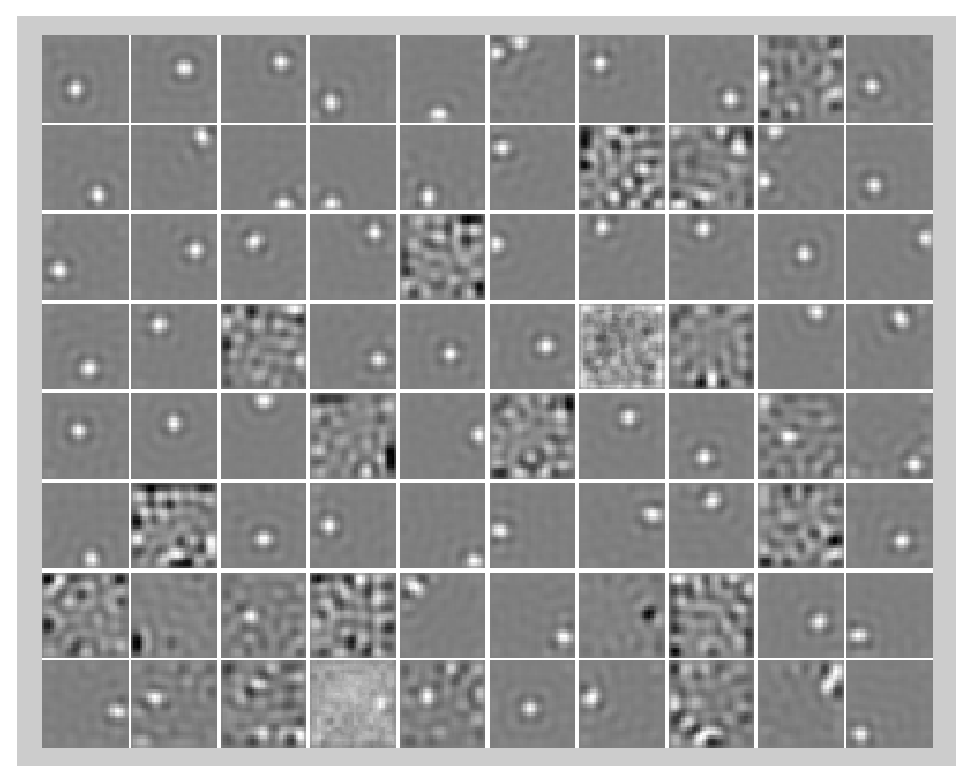
\includegraphics[width=0.4\columnwidth]{eps/center_surround}
\caption{Layer one center-surround filters learned by the neural network}
\label{fig:center_surround}
\vspace{-0.3cm}
\end{figure}

With a pre-trained (layer-wise) auto-encoder, a logistic classifier is trained on the second layer features to produce an accuracy of 82.7\% accuracy, compared with the reported 93\%. Looking at the reconstruction objectives, the two-layer network has yet large reconstruction errors (2.5e6 as compared to 1.5e6). After optimizing the two-layer network, reconstruction visualizations are much better, see Figure \ref{fig:reconstructions}, and a linear classifier is able to produce 87.5\% accuracy on discriminating numerosities below and above 16. Further I classified the same data with reference number 8, and the accuracy becomes 94\%, Zorzi et. al. did not specify their 93\% result was on reference number 8 or 16. 

\begin{figure}[tbh]
\centering
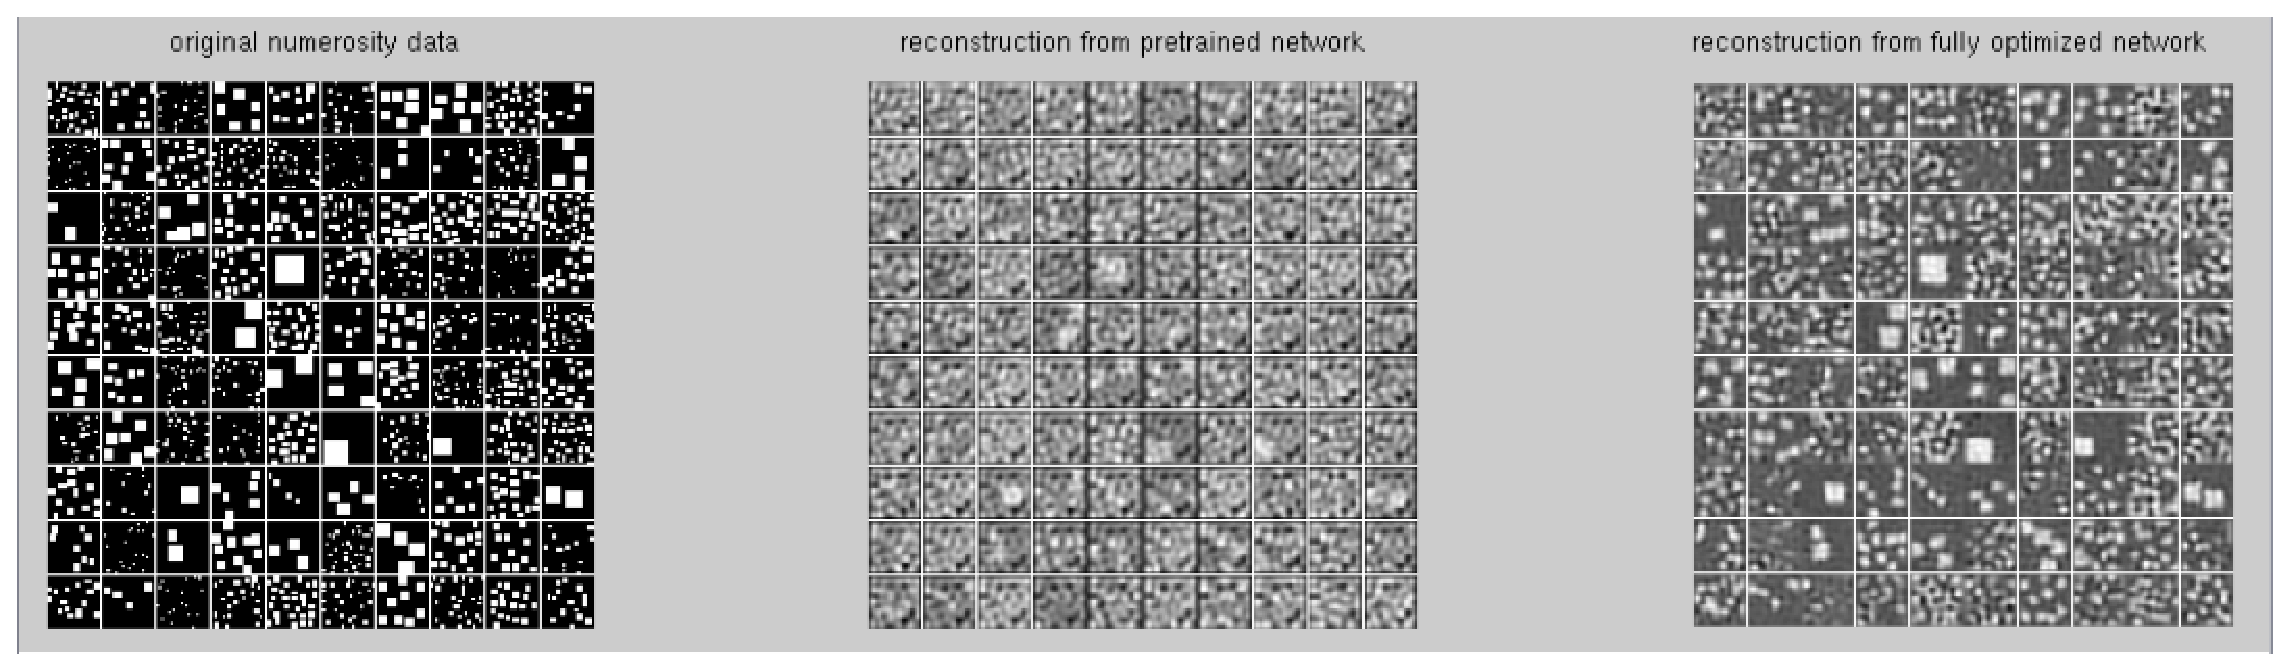
\includegraphics[width=1\columnwidth]{eps/reconstructions}
\caption{Reconstructions made by the deep auto-encoder}
\label{fig:reconstructions}
\vspace{-0.3cm}
\end{figure}

As a starting model, the deep auto-encoder seems to be able to nearly replicate Zorzi's model. 
\subsection{Denoising Auto-encoders and whitening}
I did experiments adding noise to the training process, it turns out that unless the noise level is carefully selected on a very fine-scale (adding a tiny bit of noise), results did not improve (87.8\% at best). I also tried whitening. After whitening, the first layer weights could not converge to center-surround filters, and classification accuracy dropped. 

\subsection{Weber ratio}
To reproduce Weber ratio using a sigmoid fit, I trained the classifier and produced results for reference numbers 8, 16. The resulting plot is shown in Figure~\ref{fig:w_fit}. It took some googling to find how to find the weber ratio, but it turns out we need to fit a error function (sigmoid-shaped) to the data. 

\begin{figure}[tbh]
\centering
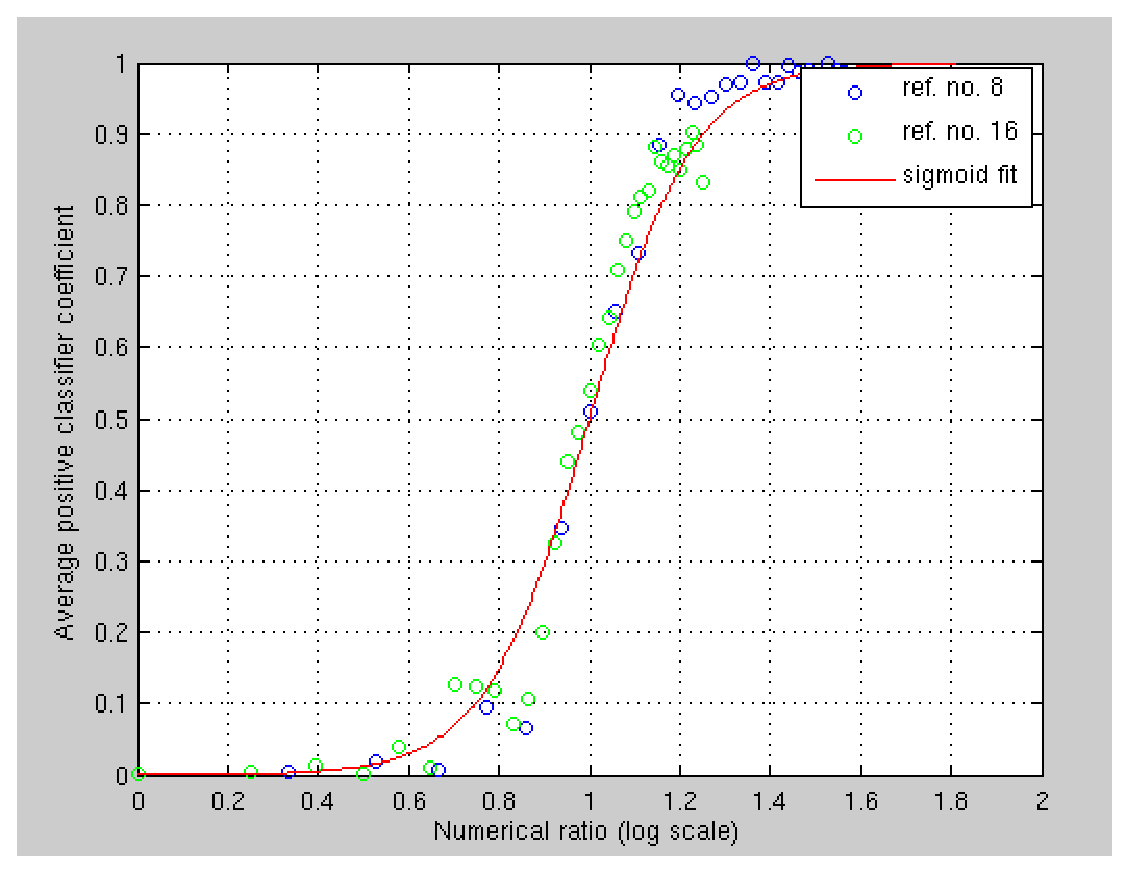
\includegraphics[width=0.5\columnwidth]{eps/w_fit}
\caption{Numerosity comparison using deep auto-encoder}
\label{fig:w_fit}
\vspace{-0.3cm}
\end{figure}

\subsection{Regression experiment}

\section{Developmental progression of weber ratio}
There has been behavioral psychology evidence that humans progressively improve their abilities to discriminate numbers. In other words, weber ratio for telling apart numbers increase consistently as one grows up. Here we perform an experiment to simulate the development progression using the deep auto-encoder, and observe the changes in weber ratio.

The details of the experiment is as follows: we apply the same deep auto-encoder as in the past sections. To simulate development progress, we perform stochastic gradient descent on the network. More specifically, since the deep network should be learned progressively, we apply the following two experiment scenarios: 
[1] Using stochastic gradient descent, we train the first and second layers iteratively, and observe the changes in weber ratio as optimization progresses. By iteratively, we mean that once a gradient step is taken on layer one, it is kept fixed before a gradient step is taken on layer 2, and so on.

[2] Using stochastic gradient descent, we first train the first layer auto-encoder, and observe changes in the weber ratio as optimization progresses. Then, we train the second layer. While adding these features to the classifier, we observe changes in the weber ratio as optimization progresses. 

{\small \bibliographystyle{ieee} \bibliography{cogsci}}
\end{document}
